\chapter{Literature Review}
\label{chapter:literature-review}

\section{Waterfall Model}
\label{sec:waterfall-model}

The waterfall model is one of the oldest and most well-known software development methodologies and was initially proposed by Winston W. Royce in 1970 \cite{royce70}. The model is characterized by its linear and sequential approach to project management \cite{Novianti2023}. Each phase must be completed before moving on to the next, and it is particularly well-suited for projects with well-defined and stable requirements.

The original waterfall model, as outlined by Royce, consisted of seven phases: System Requirements, Software Requirements, Analysis, Program Design, Coding, Testing, and Operations \cite{royce70}. However, over time, variations of the model have emerged. Hausen \cite{Hausen} mentioned that the most commonly recognized version includes five phases: Requirements Analysis, Design, Coding, Testing, and Maintenance.

One advantage of the waterfall model is its simplicity, ease of understanding, and implementation \cite{Sunardi2020}. It provides a clear structure and allows for a step-by-step progression through the development process \cite{Sunardi2020}. Rachma and Muhlas \cite{Rachma2022} argue that the waterfall model is particularly well-suited for projects that involve generic software or systems that provide services to buyers.

However, the waterfall model has also been criticized for its limitations. Zahia et al. \cite{Zahia14} argue that this model is best suited for hardware production and may overlook the unique characteristics of software development. Yahya and Maidin \cite{Yahya2023} stated that the waterfall model does not allow for flexibility or adaptability during the development process, which means that once a stage is completed, it is difficult to make changes or return to a previous stage. This lack of flexibility can be problematic when uncertainties arise or when there is a need for iterative development.

Figure \ref{fig:waterfall-model} shows the waterfall model that will be utilized for this project.

\begin{figure}[!ht]
    \centering
    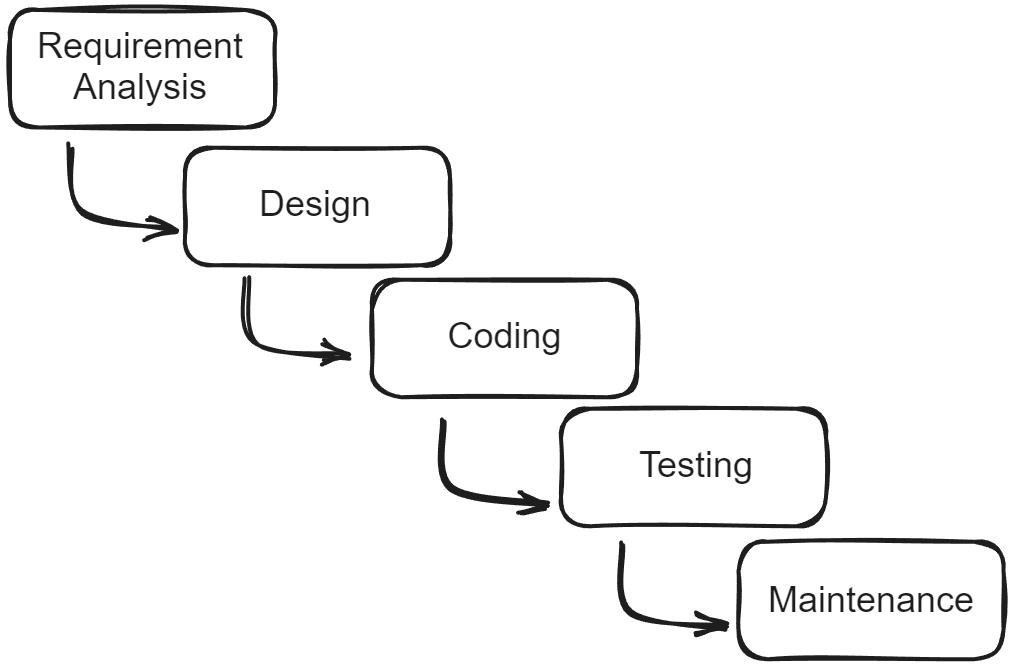
\includegraphics[width=0.65\textwidth]{texs/Part2/chapter1/image/waterfall.png}
    \caption{Waterfall Model}
    \label{fig:waterfall-model}
\end{figure}


\section{Model-View-Controller}
\label{sec:model-view-controller}

The Model-View-Controller (MVC) architecture is a design pattern commonly used in software development to separate the concerns of an application into three distinct components: the model, the view, and the controller \cite[47]{Garca2023}. The model represents the data and business logic of the application, the view is responsible for presenting the data to the user, and the controller handles user input and updates the model and view accordingly \cite{sarker14}.

The MVC architecture offers several benefits for software development. Firstly, it promotes code reusability by separating the different aspects of the application \cite{sarker14}. Additionally, MVC allows for multiple representations of the same information, creating different views for different user interfaces \cite{sarker14}. This flexibility is advantageous in interactive applications where users may have different preferences or requirements.

Another significant advantage of MVC is that it allows for the separation of concerns \cite{Stepien}. By isolating the data, business logic, and presentation layers, developers can better understand and modify each component without affecting the others. This modularity improves the maintainability and scalability of the application, as changes can be made to one component without impacting the entire system \cite{Kozon_2023}.

The application will utilize the MVC pattern as its backbone. Further implementation details will be discussed in the following chapter. Figure \ref{fig:mvc} shows the MVC architecture being used for this project.

\begin{figure}[!ht]
    \centering
    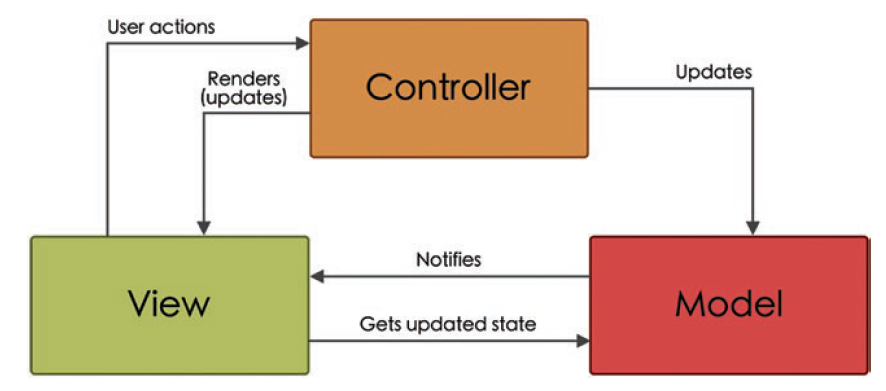
\includegraphics[width=0.65\textwidth]{texs/Part2/chapter1/image/mvc.png}
    \caption{Model-View-Controller Architecture \cite[46]{Garca2023}}
    \label{fig:mvc}
\end{figure}